\documentclass{beamer}
\usetheme{Frankfurt}
\usecolortheme{beaver} 

% Remove navigation symbols
\setbeamertemplate{navigation symbols}{}

% Change bullet points
\setbeamertemplate{itemize items}[square]


% Add page number to top bar

\newcounter{num}
\newcounter{totalnum}

\def\pagenumbers#1#2{\expandafter\ifnum#1>#2\relax\else{\large#1}/#2\fi}

\makeatletter
\defbeamertemplate*{headline}{my smoothbars theme}
{%
  \setcounter{num}{\insertframenumber}%
  \addtocounter{num}{-1}%
  \setcounter{totalnum}{\inserttotalframenumber}%
  \addtocounter{totalnum}{-1}%
  \pgfuseshading{beamer@barshade}%
  \ifbeamer@sb@subsection%
    \vskip-9.75ex%
  \else%
    \vskip-7ex%
  \fi%
  \begin{beamercolorbox}[ignorebg,ht=2.25ex,dp=3.75ex]{section in head/foot}
    \insertnavigation{.9\paperwidth}\hfill\raisebox{-2ex}{\pagenumbers{\thenum}{\thetotalnum}}\hspace{.5em}
  \end{beamercolorbox}%
  \ifbeamer@sb@subsection%
    \begin{beamercolorbox}[ignorebg,ht=2.125ex,dp=1.125ex,%
      leftskip=.3cm,rightskip=.3cm plus1fil]{subsection in head/foot}
      \usebeamerfont{subsection in head/foot}\insertsubsectionhead
    \end{beamercolorbox}%
  \fi%
}%
\makeatother

% List of what areas setbeamercolor can change
% 
% abstract
% abstract title
% alerted text
% author
% author in head/foot
% author in sidebar
% background
% background canvas
% bibliography entry author
% bibliography entry location
% bibliography entry note
% bibliography entry title
% bibliography item
% block body
% block body alerted
% block body example
% block title
% block title alerted
% block title example
% button
% button border
% caption
% caption name
% date
% date in head/foot
% date in sidebar
% description item
% enumerate item
% enumerate subitem
% enumerate subsubitem
% example text
% fine separation line
% footline
% framesubtitle
% frametitle
% frametitle right
% headline
% institute
% institute in head/foot
% institute in sidebar
% item
% item projected
% itemize item
% itemize subitem
% itemize subsubitem
% itemize/enumerate body
% itemize/enumerate subbody
% itemize/enumerate subsubbody
% local structure
% logo
% lower separation line foot
% lower separation line head
% math text
% math text displayed
% math text inlined
% middle separation line foot
% middle separation line head
% mini frame
% navigation symbols
% navigation symbols dimmed
% normal text
% normal text in math text
% normal text in math text
% page number in head/foot
% palette primary
% palette quaternary
% palette secondary
% palette sidebar primary
% palette sidebar quaternary
% palette sidebar secondary
% palette sidebar tertiary
% palette tertiary
% part name
% part title
% qed symbol
% quotation
% quote
% section in head/foot
% section in sidebar
% section in sidebar shaded
% section in toc
% section in toc shaded
% section name
% section number projected
% section title
% separation line
% sidebar
% sidebar left
% sidebar right
% structure
% subitem
% subitem projected
% subsection in head/foot
% subsection in sidebar
% subsection in sidebar shaded
% subsection in toc
% subsection in toc shaded
% subsection name
% subsection number projected
% subsection title
% subsubitem
% subsubitem projected
% subsubsection in head/foot
% subsubsection in sidebar
% subsubsection in sidebar shaded
% subsubsection in toc
% subsubsection in toc shaded
% subsubsection number projected
% subtitle
% title
% title in head/foot
% title in sidebar
% titlegraphic
% titlelike
% upper separation line foot
% upper separation line head
% verse

% CERN blue is Pantone 286 = RGB 56 97 170, defined as cern@blue below

\definecolor{cern@ltblue}{rgb}{0.415686,0.611765,0.964706} % RGB 106 156 246
\definecolor{cern@blue}  {rgb}{0.219608,0.380392,0.666667} % RGB  56  97 170
\definecolor{cern@dkblue}{rgb}{0.082353,0.184314,0.364706} % RGB  21  47  93

% Complimentary colours

\definecolor{cern@ltcomp}{rgb}{0.666667,0.525490,0.219608} % RGB 170 134  56
\definecolor{cern@dkcomp}{rgb}{0.364706,0.266667,0.047059} % RGB  93  68  12

\setbeamercolor{title}                   {bg=cern@blue,fg=white}
\setbeamercolor{frametitle}              {bg=cern@blue,fg=white}
\setbeamercolor{section in head/foot}    {bg=cern@ltblue,fg=white}
\setbeamercolor{structure}               {fg=cern@dkcomp}
\setbeamercolor{bibliography entry title}{fg=cern@ltblue}

%
% Get packages that we need
%

% Change fonts to Avenir
% Note: need to compile with xelatex to use this package
\usepackage{fontspec}
\setsansfont{AvenirLTStd-Book}

%\usepackage[showboxes,overlay,absolute]{textpos}
\usepackage[overlay,absolute]{textpos}
\setlength{\TPHorizModule}{.01\paperwidth} % Horizontal units are percent of paper width
\setlength{\TPVertModule}{.01\paperwidth}  % Make vertical units equal to horizontal units
\textblockorigin{.5\paperwidth}{4.25ex}

% Headings within slides
\usepackage{xcolor}

\usepackage{tabularx}
\usepackage{enumitem}
\setitemize{label=\usebeamerfont*{itemize item}%
  \usebeamercolor[fg]{itemize item}
  \usebeamertemplate{itemize item}}

\newcommand\colhead[1]{\fontspec{Humanst521 BT}\textcolor{cern@dkblue}{\small\textbf{#1}}}

\newcommand\boxhead[1]{%
  \par\begin{center}
  \fontspec{Humanst521 BT}\textcolor{cern@dkblue}{\textbf{#1}}
  \end{center}\par}

% Shortcuts to handle 1st, 2nd, 3rd, 4th
\usepackage{relsize}
\newcommand{\squared}{\ensuremath{^{\textsf{2}}} }
\newcommand{\superscript}[1]{\ensuremath{^{\textsf{\smaller #1}}}}
\newcommand{\subscript}[1]{\ensuremath{_{\textsf{\smaller #1}}}}
\newcommand{\st}[0]{\superscript{st} }
\newcommand{\nd}[0]{\superscript{nd} }
\newcommand{\rd}[0]{\superscript{rd} }
\renewcommand{\th}[0]{\superscript{th} }

%
% Citation aliasing
%

\let\oldbibitem=\bibitem
\renewcommand{\bibitem}[2][]{\label{mybib#2}\oldbibitem[#1]{#2}}
%\newcommand\citealias[2]{\hyperlink{bib#1}{#2}\phantom{\cite{#1}}}
%\newcommand\citealias[2]{\cite[#2]{#1}}
\newcommand\citealias[2]{\hyperlink{mybib#1}{#2}\phantom{\cite{#1}}}

\newcommand\x{$\times$}
\usepackage{setspace}

\usepackage{listings}
\lstset{basicstyle=\ttfamily\color{cern@dkcomp}}
\newcommand{\code}[1]{{\ttfamily\color{cern@dkcomp}#1}}

\begin{document}
%%
%% Title Page
%%

{
\setbeamertemplate{headline}{}
\begin{frame}
\begin{center}
\vspace{-4ex}

\includegraphics[width=0.25\textwidth]{../Logo/cern-logo-blue}\\[4ex]
\color{cern@dkblue}
\begin{spacing}{1.0}
   {\fontsize{17}{22}\fontspec{Humanst521 BT}Introduction to the}\\[2ex]
   {\fontsize{17}{22}\fontspec{Humanst521 BT}CERN Tape Archive (CTA)}\\[4ex]
\end{spacing}
\color{cern@dkcomp}
   {\large Michael Davis, for the CTA Team}\\[2ex]
   {22 July 2020}
\end{center}
\end{frame}
}

\color{cern@dkblue}

%%
%% SECTION 1
%%

\section{Use Cases}
\subsection{}

\begin{frame}{EOS+CTA}{}
   \centering
   
\includegraphics[width=\textwidth]{images/EOS+CTA_Logo}

   \vspace{1cm}
   {\LARGE\centering CTA is the tape back-end to EOS}
\end{frame}

\begin{frame}{Changing Use Cases for Archival Storage}{1. Scaling up for Run 3 and HL--LHC}
\begin{textblock}{98}[0.5,0](0,9) % {block width} (coords)
   \centering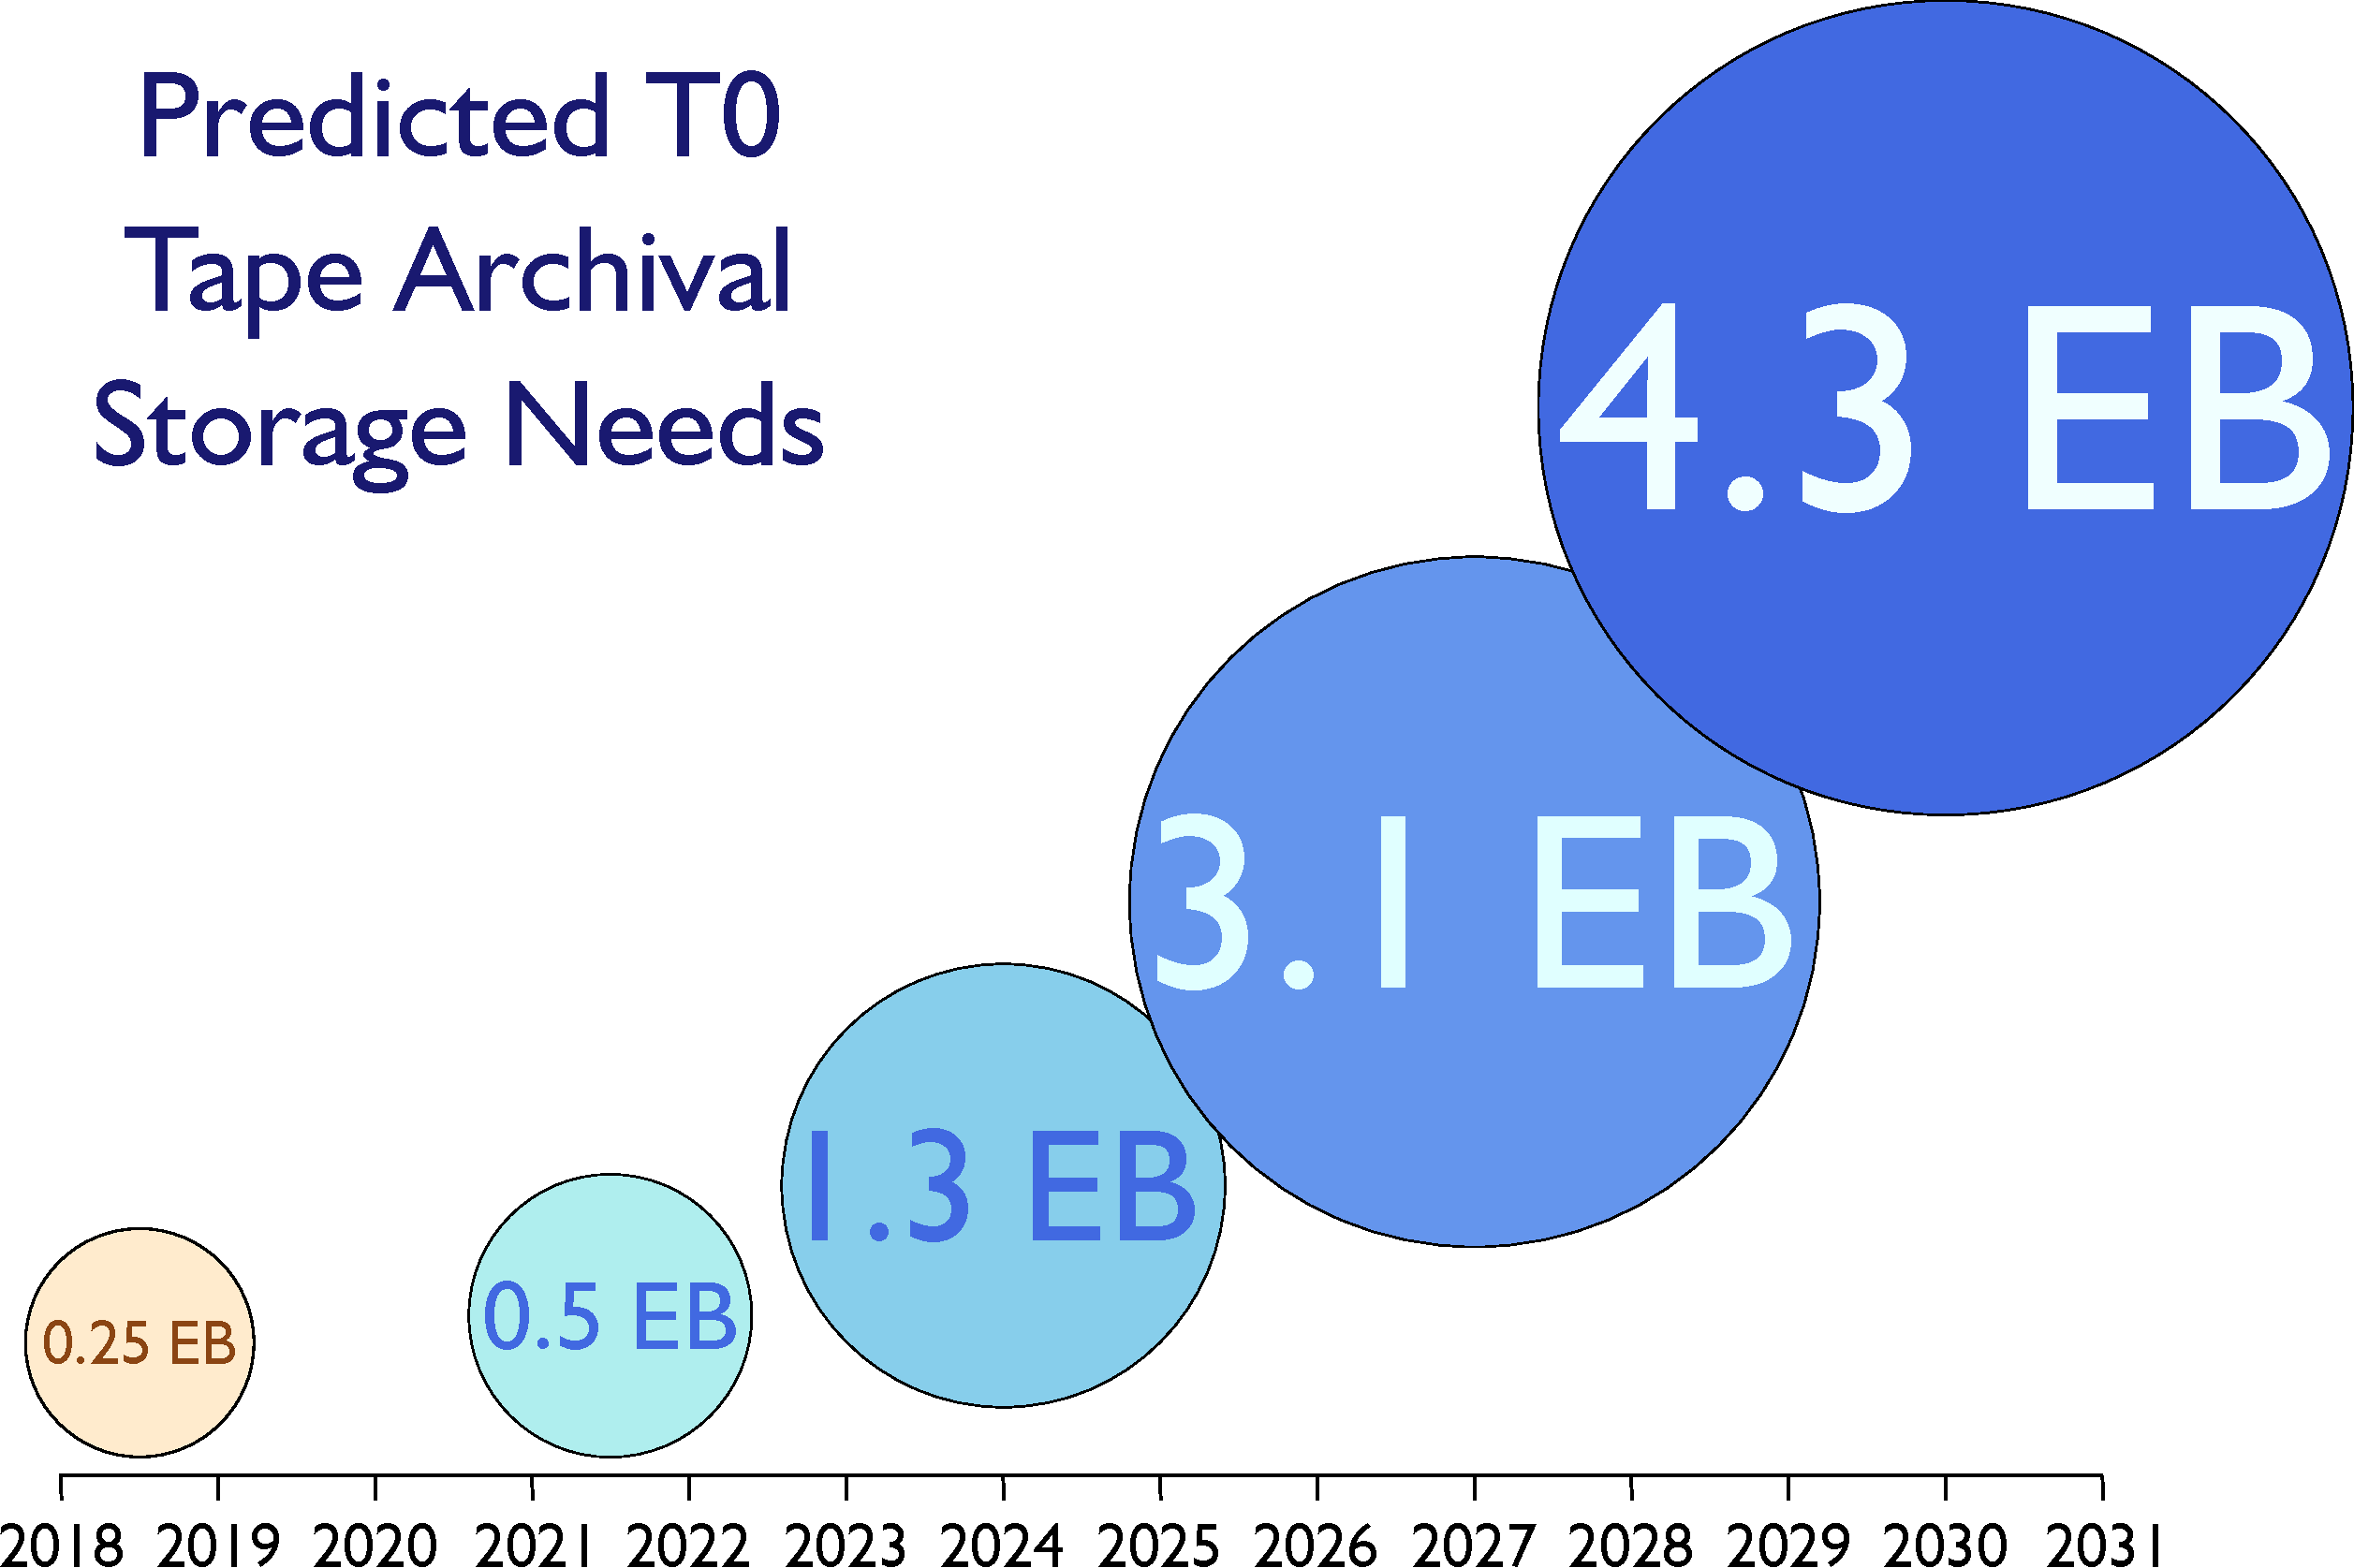
\includegraphics[width=0.9\textwidth]{images/Storage}
   %{\centering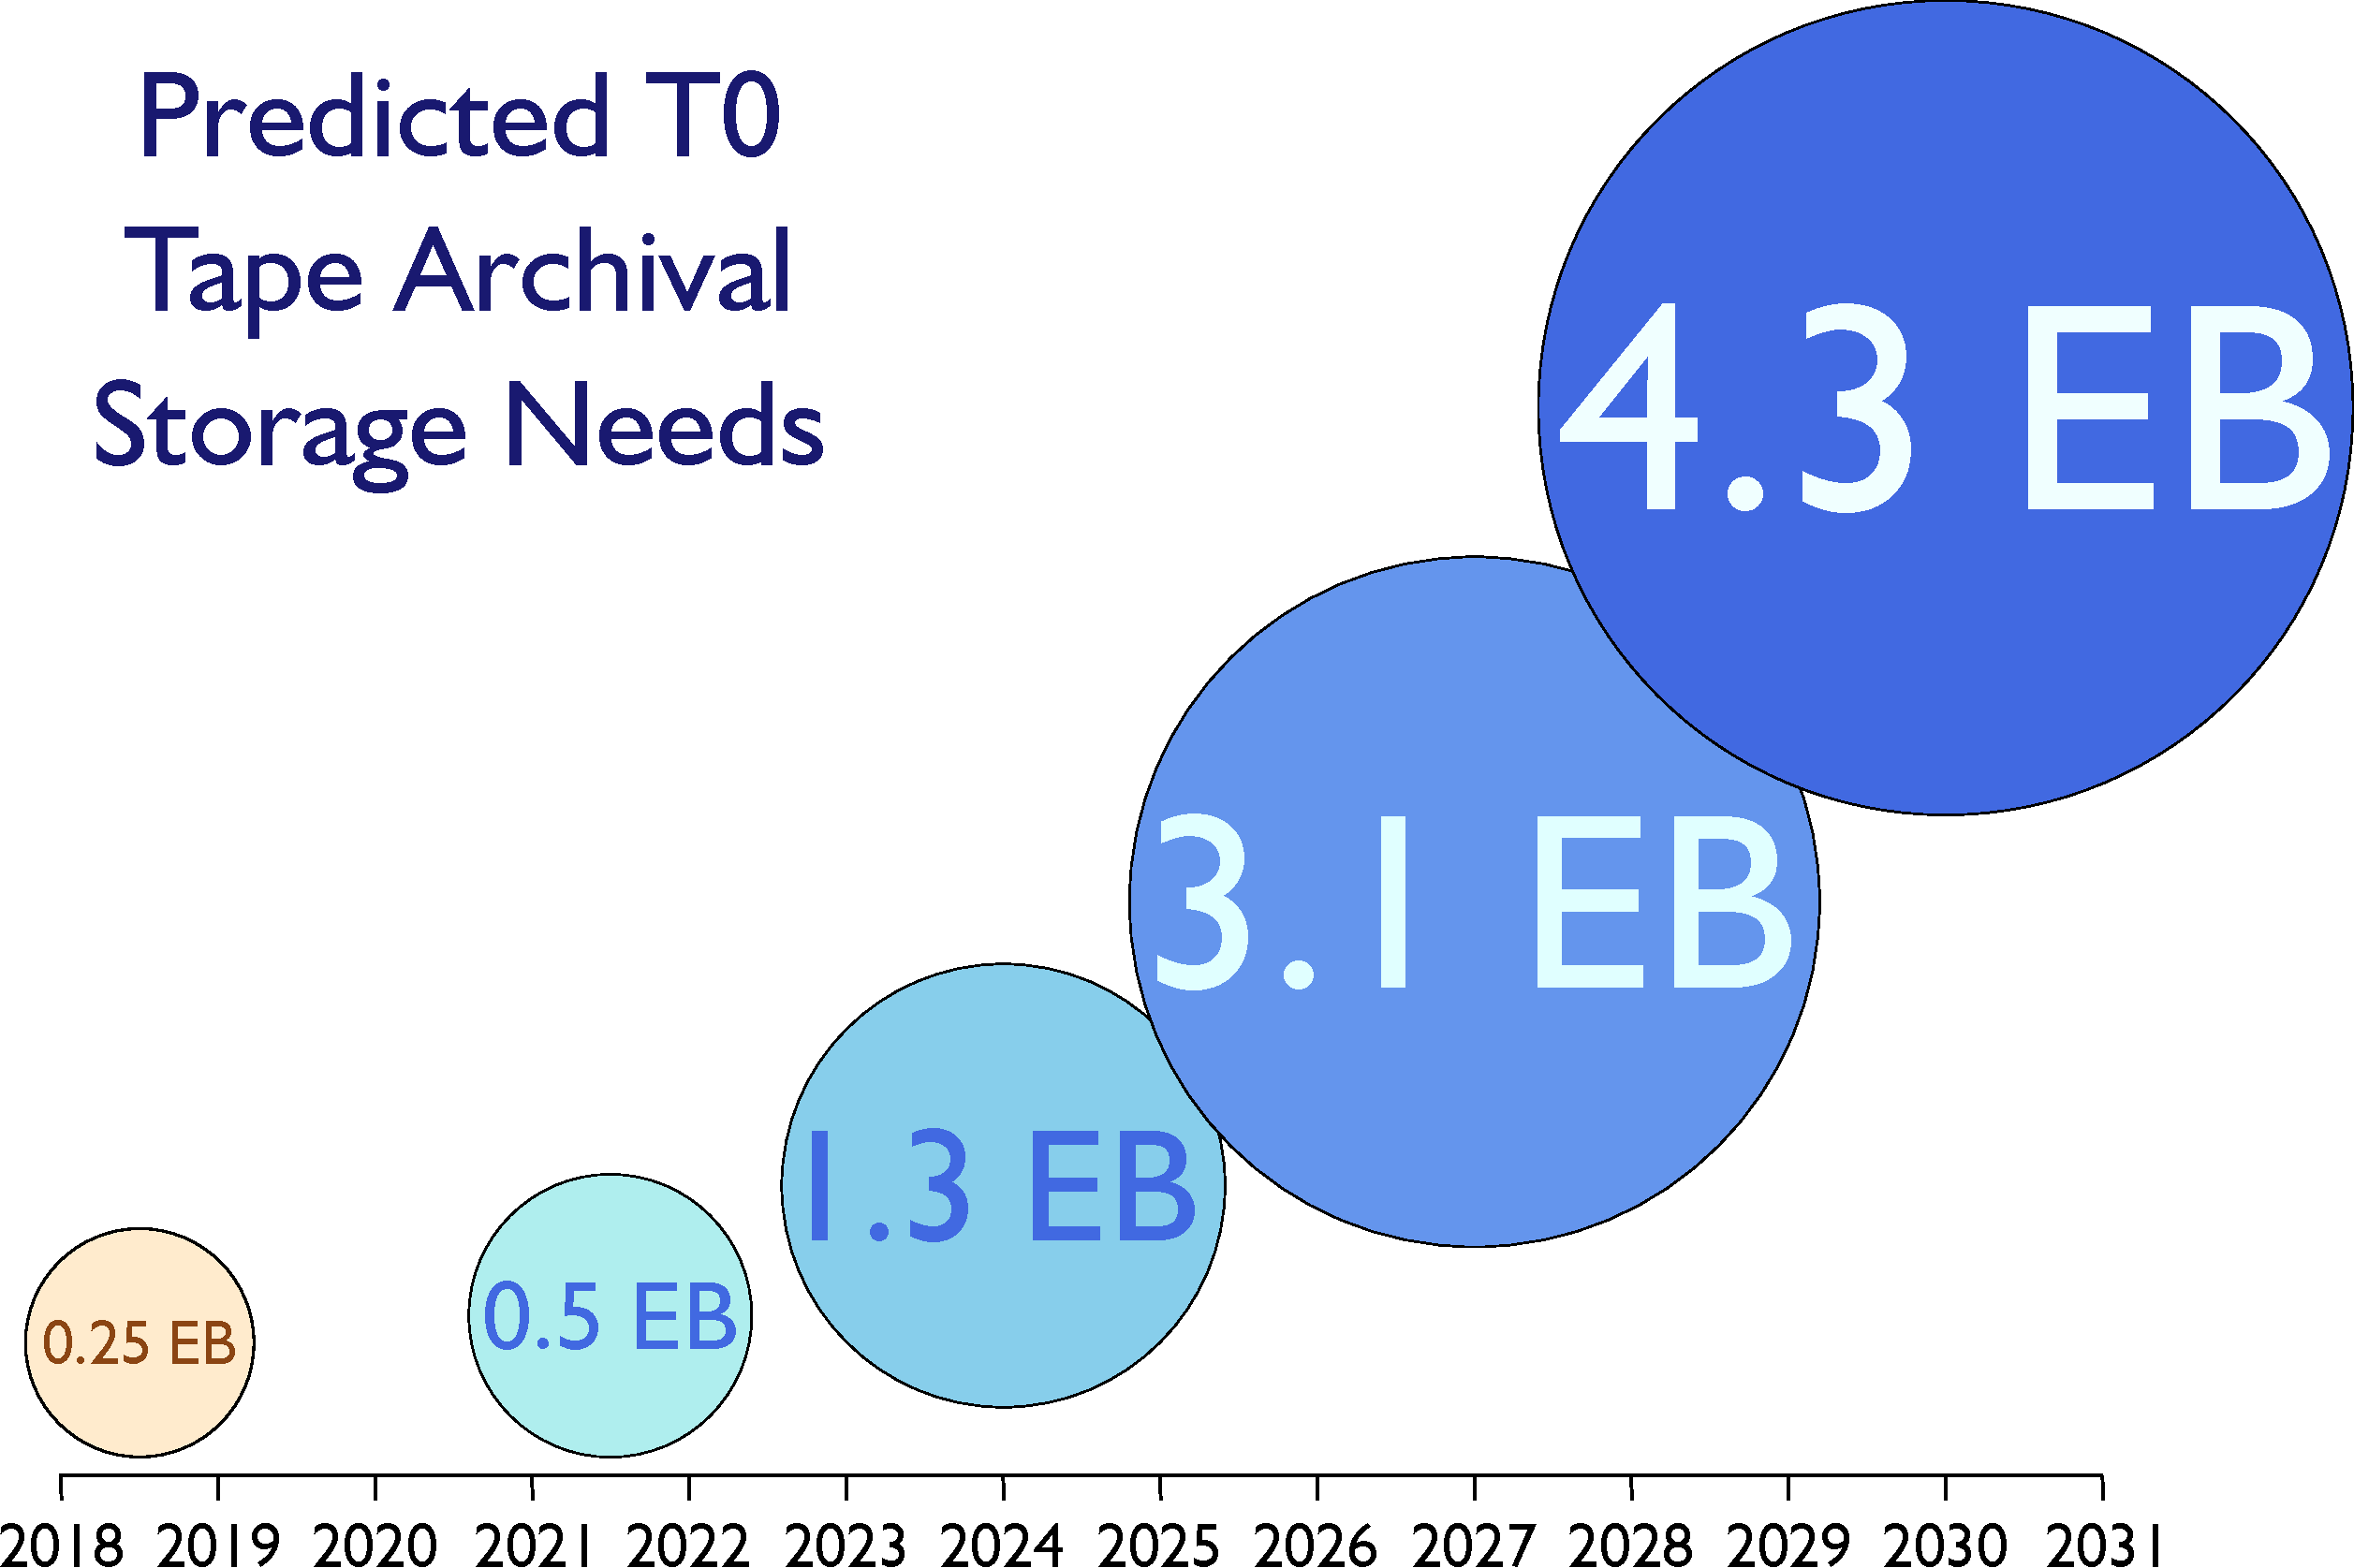
\includegraphics[width=0.75\textwidth]{images/Storage}\\[1.7ex]}
   %\leftskip1em\rightskip\leftskip\scriptsize\color{black}Source:
   %\href{http://iopscience.iop.org/article/10.1088/1742-6596/664/4/042006/meta}{\color{cern@ltblue}Experiences
   %and challenges running CERN's high capacity tape archive}\\
   %\leftskip5.1em Germ\'{a}n Cancio \textit{et al}, IOP 2015
\end{textblock}
\end{frame}

\begin{frame}{Changing Use Cases for Archival Storage}{2. Data for online analysis stored on tape (``Data Carousel'')}
\begin{textblock}{100}[0.5,0](0,8) % {block width} (coords)
   \includegraphics<1>[width=\textwidth]{images/DataCarousel.png}
   \includegraphics<2>[width=\textwidth]{images/DataCarouselChart.png}\\[2ex]
   \leftskip1em\rightskip\leftskip\scriptsize\color{black}Source:
   \href{https://indico.cern.ch/event/732181/contributions/3019046/}{\color{cern@ltblue}Tape Usage},
   Xin Zhao (Brookhaven National Laboratory), ADC Technical Coordination\\
   \leftskip5.1em Board Meeting, 28 May 2018
\end{textblock}
\end{frame}

\begin{frame}{Data Archival at CERN/WLCG}
\begin{itemize}
   \item The custodial copy of all CERN physics data is stored on tape here at Tier-0.
   \item Additional copies of the data are distributed across the grid. Tier-1s also provide tape archival storage.
      % T0 Meyrin Data Centre is custodial copy of the physics data 350 PB, T1s can be around 20%
   \item The current Tier-0 production tape archival system (\href{http://castor.web.cern.ch/}{\color{cern@blue}CASTOR}) will be progressively replaced by EOS+CTA.
   \item Many different tape systems in use across the Tier-1s. Likely consolidation in the coming years.
\end{itemize}
\end{frame}

\section{CTA Architecture}
\subsection{}

\begin{frame}{CASTOR Architecture}
\begin{textblock}{98}[0.5,1](0,68.5) % {block width} (coords)
   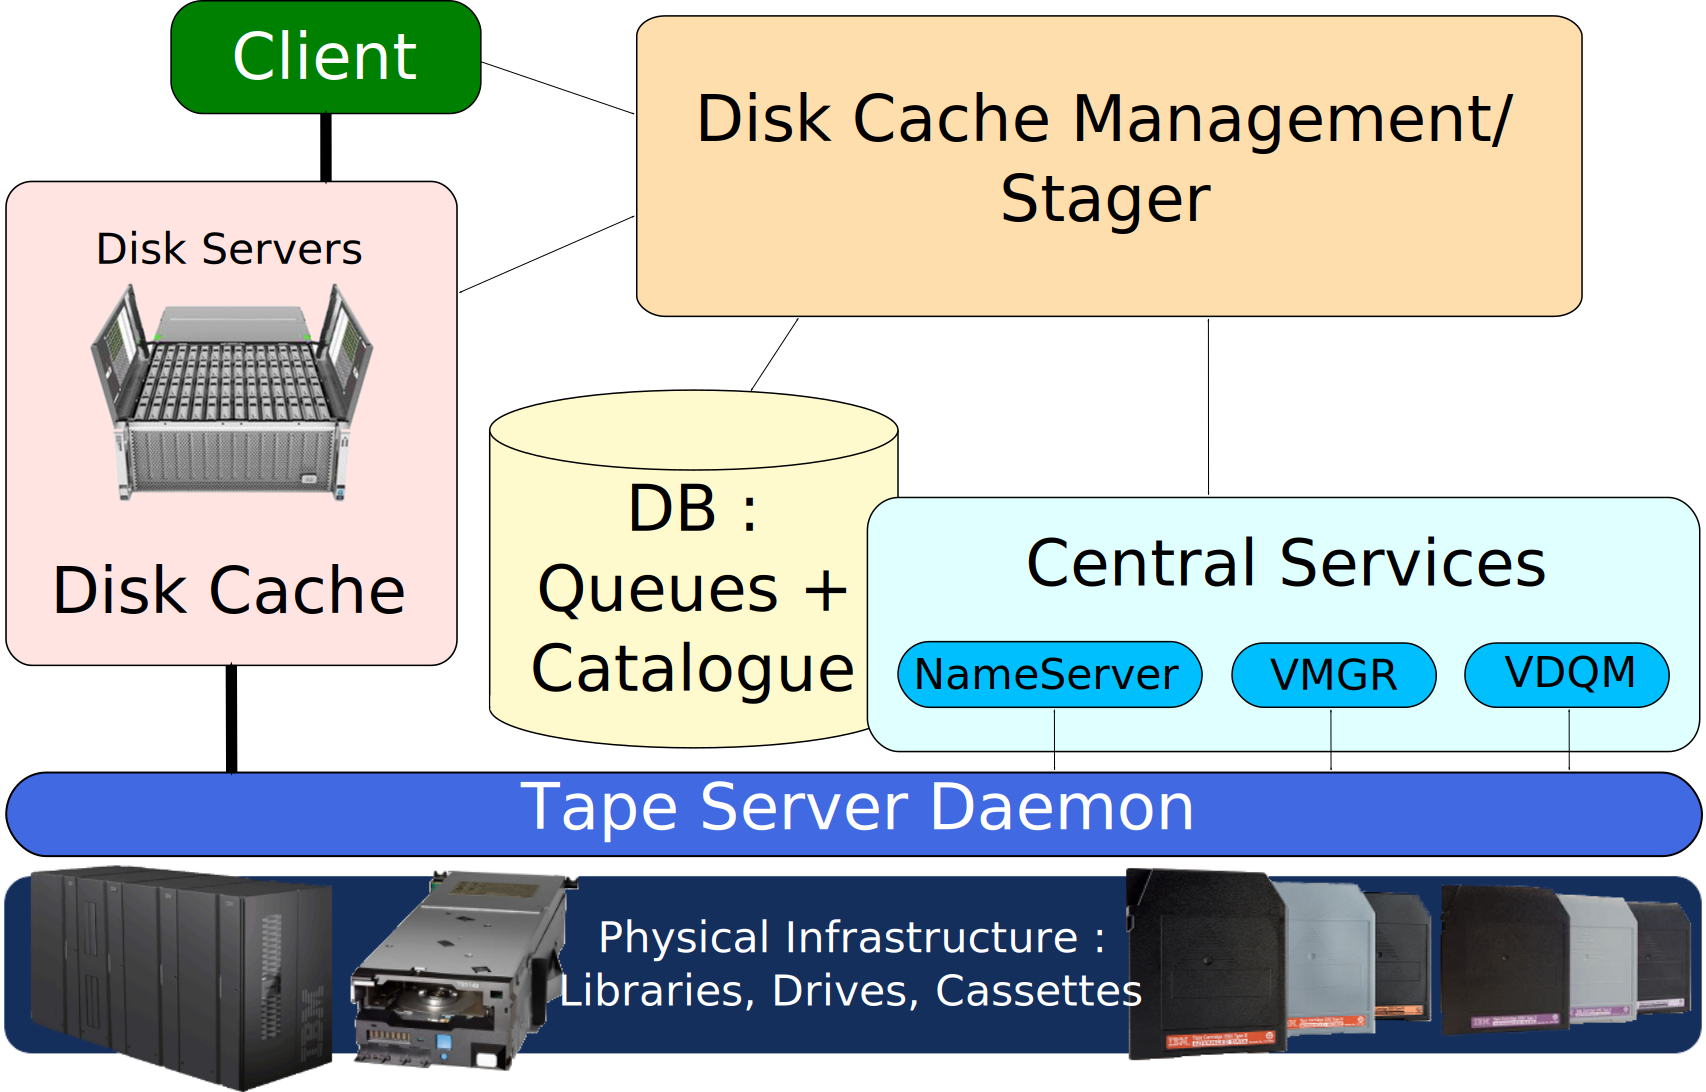
\includegraphics[width=\textwidth]{images/CASTOR_Arch}
\end{textblock}
\end{frame}

\begin{frame}{CTA Architecture}
\begin{textblock}{98}[0.5,1](0,68.5) % {block width} (coords)
   %\includegraphics<1>[width=\textwidth]{images/CTA_Arch1}
   %\includegraphics<2>[width=\textwidth]{images/CTA_Arch2A}
   %\includegraphics<3>[width=\textwidth]{images/CTA_Arch3}
   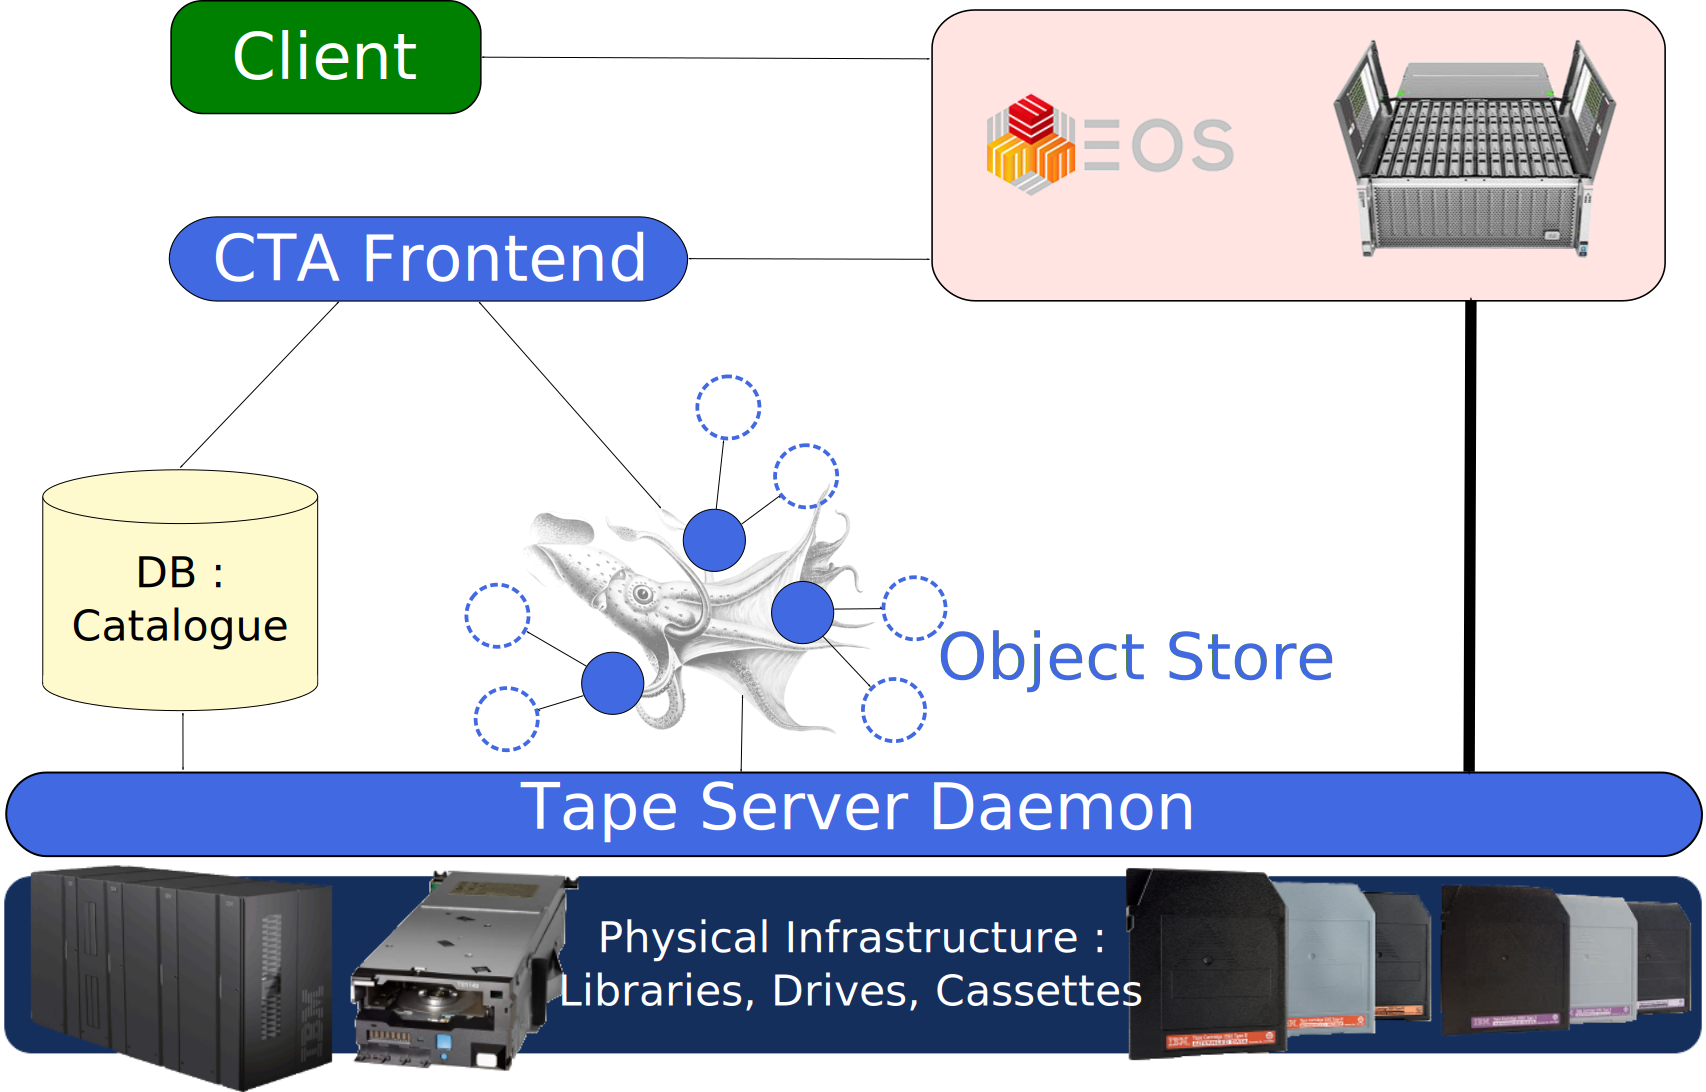
\includegraphics[width=\textwidth]{images/CTA_Arch3A}
\end{textblock}
\end{frame}

\begin{frame}{EOS+CTA : Who Does What?}{}
   \renewcommand{\arraystretch}{1.1}
   \begin{tabularx}{\textwidth}{>{\raggedright}X>{\raggedright\arraybackslash}X}
        \multicolumn{1}{c}{\fontspec{Humanst521 BT}\color{cern@blue}Function}
      & \multicolumn{1}{c}{\fontspec{Humanst521 BT}\color{cern@blue}Provided by}\\[0.5ex]
      \hline
      File Metadata Operations & EOS (MGM/XRootD)\\
      Namespace & EOS (QuarkDB)\\
      Disk Buffer for Staging & EOS (FST)\\
      \hline
      Tape File Metadata Ops & CTA (Frontend)\\
      % CTA does not know the filename of a file. If you give it a fileid, it can tell you its size
      % and checksum, how many copies there are and which tapes the copies are stored on.
      Archive/Recall Requests & CTA (Objectstore)\\
      Tape File Catalogue & CTA (Catalogue DB)\\
      Tape Operations (libraries, drives, cassettes) & CTA (Tape Server)\\
   \end{tabularx}
% Main difference with CASTOR: EOSCTA is a pure tape system.
\end{frame}

\begin{frame}{Object Store}
\begin{textblock}{98}[0.5,1](0,68.5) % {block width} (coords)
   \includegraphics<1>[width=\textwidth]{images/ObjectStore}
\end{textblock}
\begin{textblock}{63}[0,0](-15,7) % {block width} (coords)
   \begin{itemize}
      \item Object Store is used for transient requests, queues, statuses and agents\\[2ex]
      \item No direct Inter-Process Communication\\[2ex]
      \item Resilience against crashes
      {\small
      \begin{itemize}
         \item Guaranteed coherency
         \item Agent heartbeat, garbage collection\\[2ex]
      \end{itemize}
      }
      \item Distributed architecture
      {\small
      \begin{itemize}
         \item Allows multiple redundant RADOS instances/CTA Frontends
         \item Scale-out scalability\\[2ex]
      \end{itemize}
      }
      \item No single point of failure
   \end{itemize}
\end{textblock}
\end{frame}

\begin{frame}{Database}{}
   {\Large Simplified use of relational databases}\\[2ex]
   \begin{itemize}
      \item Thanks to the CTA Object Store there are no longer any stager databases
      \item 1 CTA DB instead of 8 CASTOR DBs
   \begin{itemize}
      \item CASTOR has 3 central DBs (Nameserver, VDQM, VMGR) and 5 stager DBs (4 LHC experiments + Public)
      \item CTA has only the tape catalogue
   \end{itemize}
   \end{itemize}
\end{frame}

\begin{frame}{Database}{}
   {\Large Supported Database Back-ends}\\[2ex]
   \begin{itemize}
      \item Oracle: The current CERN production solution
      \item PostgreSQL: The future CERN production solution and recommended Tier 1 solution
      \item MySQL: Developed by IHEP China for Tier 1s
      \item SQLite: In-memory database for C++ unit tests
   \end{itemize}
\end{frame}

\begin{frame}{Tape Library Support}{}
   {\Large CTA supports SCSI}
   \begin{itemize}
   \item IBM tape libraries
   \item SpectraLogic libraries
   \item mhVTL virtual libraries
   \item Oracle libraries with an additional SCSI interface\\[4ex]
   \end{itemize}
   {\Large CTA does \textbf{not} support ACSLS}
   \begin{itemize}
   \item ACSLS is used by Oracle libraries
   \item Workaround solutions could be implemented, e.g. Tape server calls an external script
   \end{itemize}
\end{frame}

\begin{frame}{CTA Architecture}{}
   \vspace{2ex}
   {\textcolor{cern@dkblue}{\Large CTA offers the ``Best of Both Worlds''}}\\[1ex]
   \begin{itemize}
      \item User interface, file access and disk pool management ~ from EOS
      \item Tape system management from CASTOR
      \item New scalable, robust queuing system to link the two\\[4ex]
   \end{itemize}
   {\textcolor{cern@dkblue}{\Large CTA design principles}}\\[1ex]
   \begin{itemize}
      \item Simplicity
      \item Scalability
      \item Performance\\[4ex]
   \end{itemize}
   %{\leftskip1em\rightskip\leftskip\scriptsize\color{black}For more details see:
   {\scriptsize Full details:
   \href{http://iopscience.iop.org/article/10.1088/1742-6596/898/6/062013/pdf}{\color{cern@ltblue}An
   efficient, modular and simple tape archiving solution for LHC Run 3},\\
   \vspace{-0.8ex}\hspace{5.1em} Steven Murray \textit{et al.} (CERN), CHEP 2016}
   %\leftskip5.1em Board Meeting, 28 May 2018
\end{frame}

\begin{frame}{``Big EOS'' and ``Little EOS''}
\begin{columns}
	\begin{column}{0.4\textwidth}
		\begin{center}
		  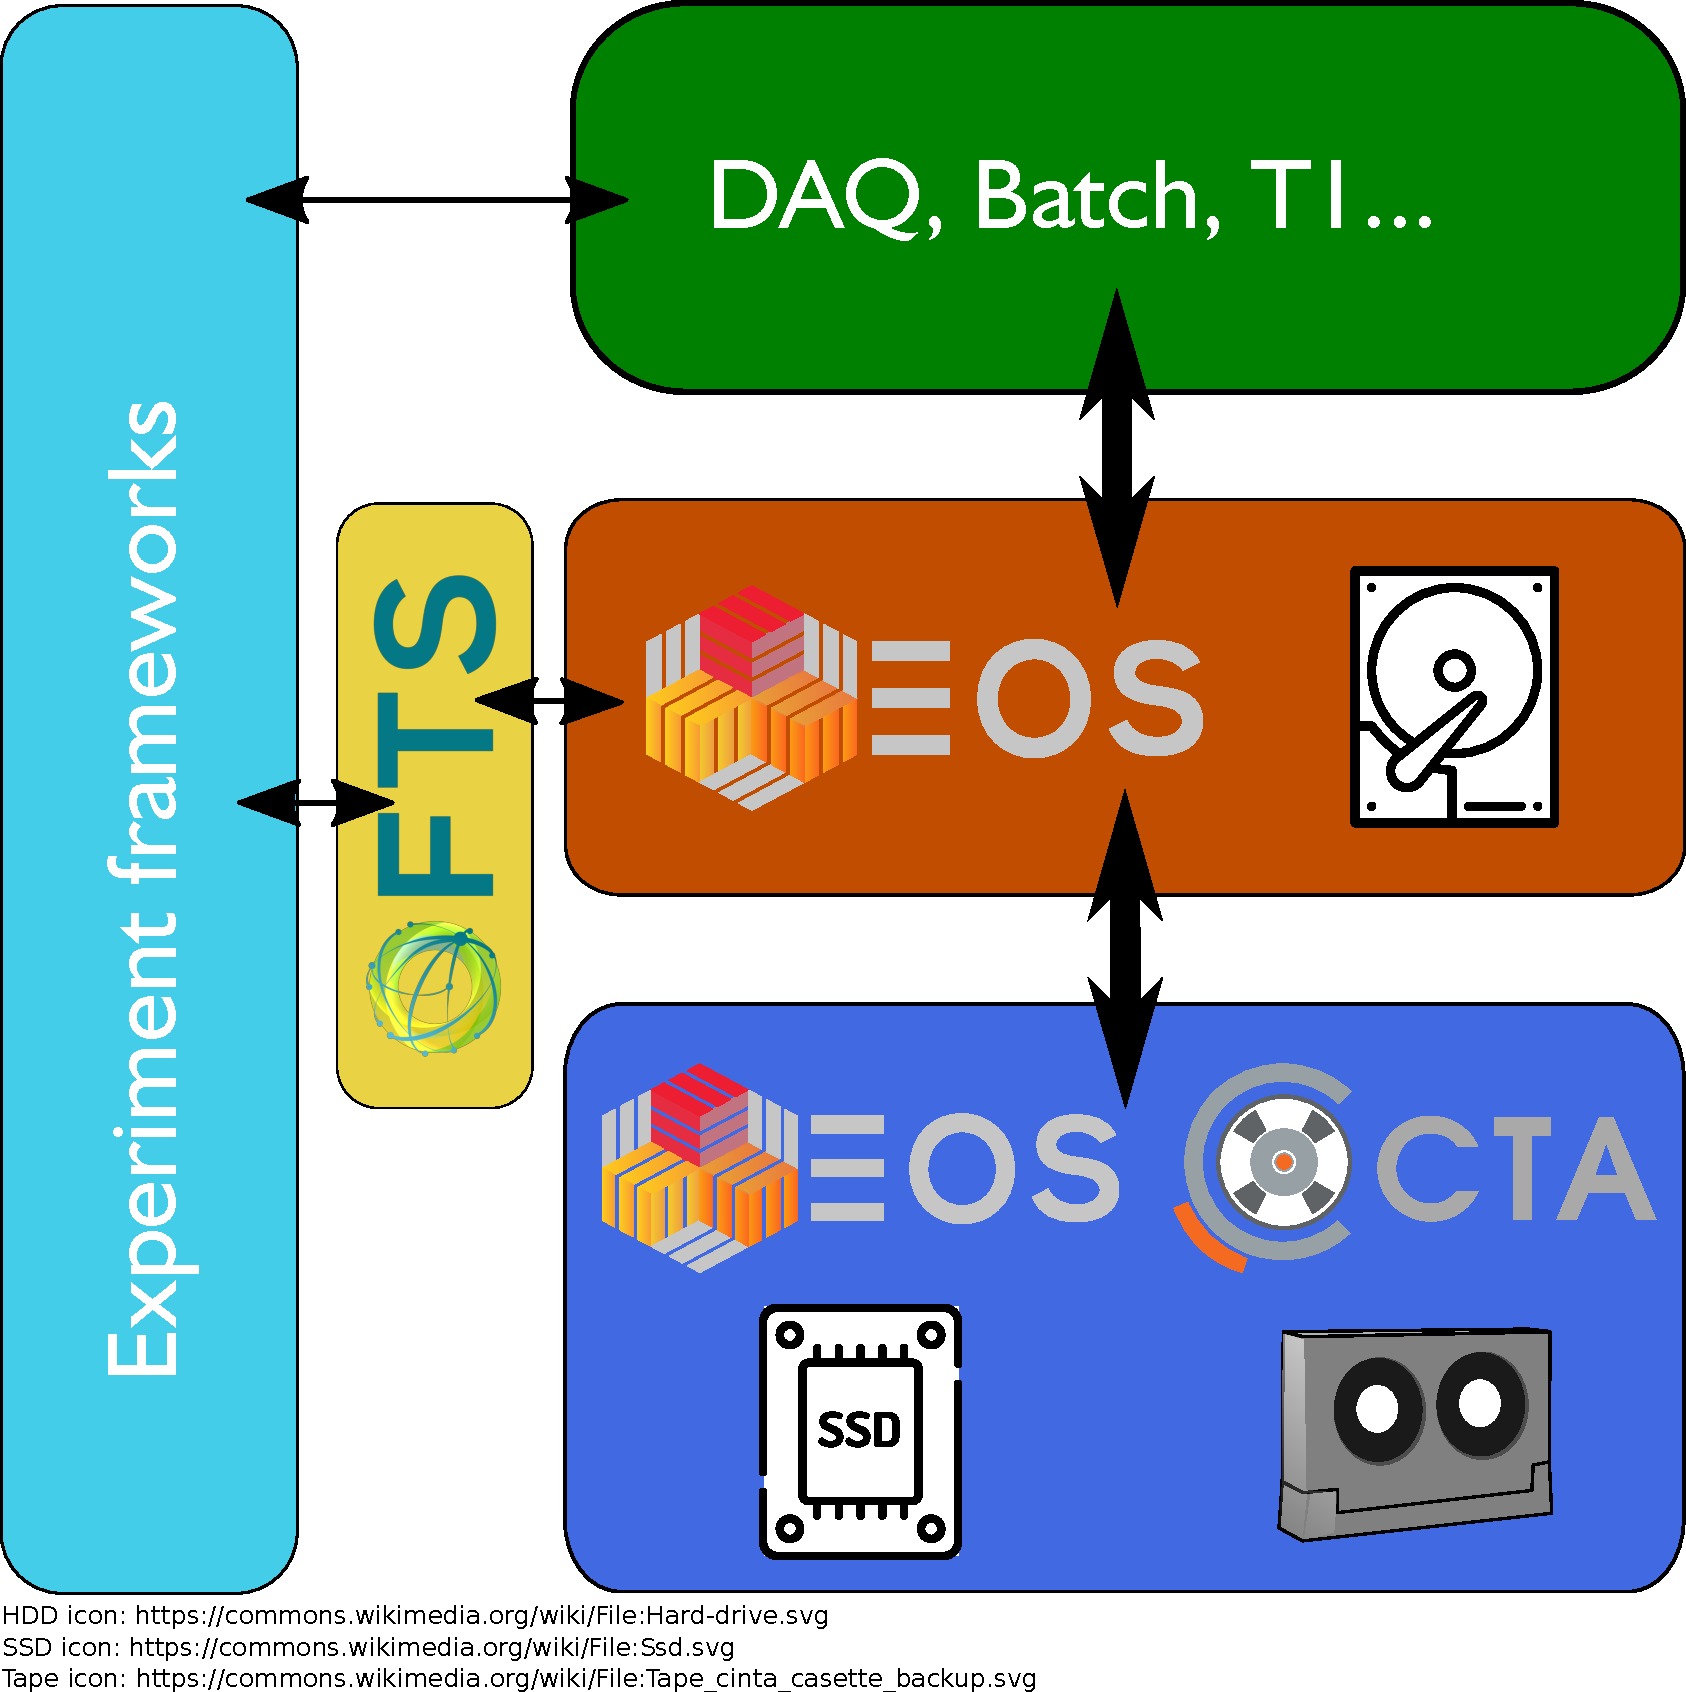
\includegraphics[width=\textwidth]{images/CTA_Deployment_model.pdf}
		\end{center}
	\end{column}
	\begin{column}{0.55\textwidth}
      ``Big EOS''
      {\small
\begin{itemize}
        \item Tens of PB of storage for physics jobs and staging to Tier-1s.
        \item File replicas have a long lifetime.
        \item Spinning disks.
\end{itemize}
      }
      ``Little EOS''
      {\small
		\begin{itemize}
        \item Small buffer for copying files to/from tape.
        \item File replicas have a very short lifetime. Deleted as soon as tape copy exists (archival) or
           copied to ``Big EOS'' (retrieval).
        \item SSDs: reduce contention and give the best price/performance ratio.
		\end{itemize}
      }
	\end{column}
\end{columns}
\end{frame}

\begin{frame}{Tape Workflows}{}
   {\small
   \begin{tabularx}{\textwidth}{p{3cm}>{\raggedright\arraybackslash}X}
      \vspace{-2cm}
\includegraphics[width=3cm]{images/Big_EOS} & \parbox[b]{\linewidth}{\begin{itemize}
         \item ``Big EOS'' is not directly connected to tape
         \item To archive/recall files, transfer them to/from \mbox{``Little EOS''} (\textit{e.g.} using \texttt{xrdcp})
      \end{itemize}}\\
      \vspace{-2cm}
\includegraphics[width=3cm]{images/Little_EOS} & \parbox[b]{\linewidth}{\begin{itemize}
         \item ``Little EOS'' has tape-backed directories
         \item Copying a file into one of these directories triggers an archival request
      \end{itemize}}\\
      \vspace{-1.95cm}\includegraphics[width=3cm]{images/CTA} & \parbox[b]{\linewidth}{\begin{itemize}
         \item CTA manages the tape queues:
         \item Archival requests streamed to mounted tape
         \item Retrieval requests grouped by tape
      \end{itemize}}\\
   \end{tabularx}
   }
\end{frame}


\end{document}
